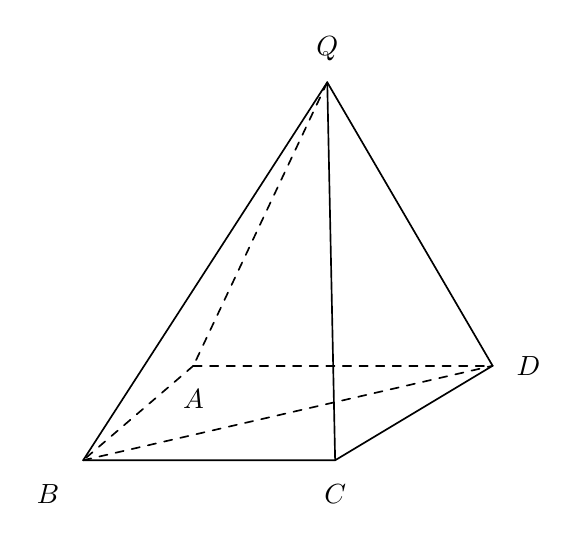
\begin{tikzpicture}[line width=0.6pt,line join=round,line cap=round]
\coordinate (Q) at (0.5,4.2);
\coordinate (A) at (-1.2,0.6);
\coordinate (B) at (-2.6,-0.6);
\coordinate (C) at (0.6,-0.6);
\coordinate (D) at (2.6,0.6);
% solid lateral edges
\draw (Q) -- (B);
\draw (Q) -- (C);
\draw (Q) -- (D);
% solid base front edges
\draw (B) -- (C) -- (D);
% hidden edges
\draw[dashed] (Q) -- (A);
\draw[dashed] (A) -- (B);
\draw[dashed] (A) -- (D);
\draw[dashed] (B) -- (D);
% labels with clearance
\node[above=4pt] at (Q) {$Q$};
\node[below=5pt] at (A) {$A$};
\node[below left=5pt] at (B) {$B$};
\node[below=5pt] at (C) {$C$};
\node[right=5pt] at (D) {$D$};
\end{tikzpicture}
